% =====================================================================
%  Chapter 5 -- Stage 2: the real circuit (bench, R_F staircase)
% =====================================================================
\chapter{Stage 2: The Real Circuit}\label{ch:stage2}
\chapterlists

The bench circuit has real noise, non-ideal components and a resistance that moves in steps of
\SI{322.6}{\ohm}. Does the $\sqrt{\lambda}$ lag survive all three?

\section{What we did}\label{sec:s2-setup}

Configuration A (\cref{fig:two-configs}a, \cref{tab:configs}): $\RF$ sweeps \SIrange{91}{101}{\kilo\ohm}
with $\Ri=\SI{47}{\kilo\ohm}$, so $G$ sweeps 2.94 to 3.15. Seventeen rates were recorded, from
\SI{103}{\ohmpersec} ($\tau=\SI{3.13}{\second}$) to \SI{9.19}{\kilo\ohm\per\second}
($\tau=\SI{35}{\milli\second}$), five cycles each. The bench oscillation runs at \SI{72.4}{\hertz} and
saturates at $\Asat=\SI{11.2}{\volt}$.

\section{What we saw}\label{sec:s2-results}

\subsection{Recordings}

At slow rates each cycle produces one flat-topped burst (\cref{fig:s2-recordings}). At
\SI{4.1}{\kilo\ohm\per\second} full size is reached just before the sweep turns back; at
\SI{7.6}{\kilo\ohm\per\second} and above the bursts are rounded, because the gain falls before growth is
complete.

\begin{figure}[!htb]
  \centering
  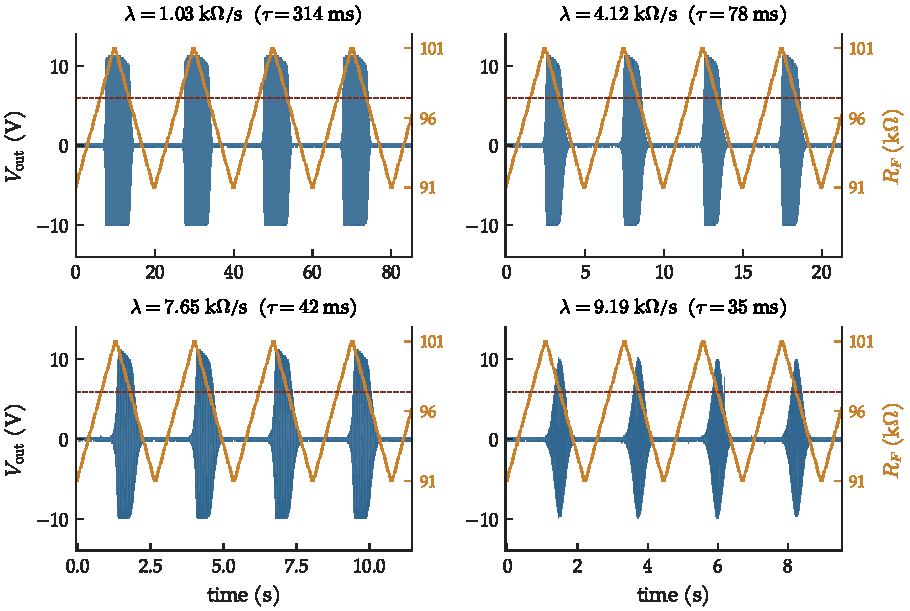
\includegraphics[width=\linewidth]{fig_s2_recordings}
  \caption[Stage 2: bench recordings at four sweep rates]{Stage 2: bench recordings. Blue: output. Orange:
  $\RF$ staircase. Dashed: measured threshold. Bursts turn from flat-topped to rounded as the rate grows.}
  \label{fig:s2-recordings}
\end{figure}

\subsection{Switching points}

\Cref{fig:s2-thresholds} collects all 17 runs. The cycle-to-cycle spread is a few tens of ohms, far
below the shifts being measured. Fitting the 13 runs below \SI{3.5}{\kilo\ohm\per\second} (switch-on)
and 14 below \SI{4.5}{\kilo\ohm\per\second} (switch-off),
\begin{align}
  \Ron  &= (\num{97313 \pm 60})\,\si{\ohm} + (\num{58.1 \pm 2.2})\sqrt{\lambda} , \label{eq:s2-on}\\
  \Roff &= (\num{97472 \pm 34})\,\si{\ohm} - (\num{31.8 \pm 1.1})\sqrt{\lambda} . \label{eq:s2-off}
\end{align}

\begin{figure}[!htb]
  \centering
  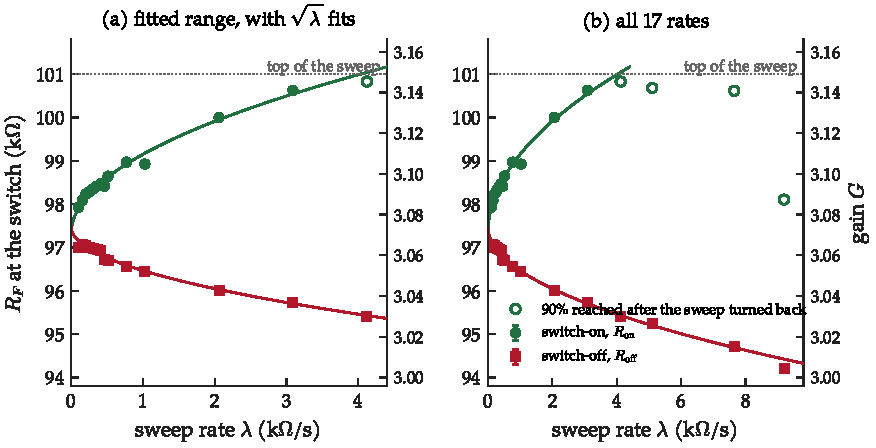
\includegraphics[width=\linewidth]{fig_s2_thresholds}
  \caption[Stage 2: switching points on the bench]{Stage 2: (a)~fitted range with
  \cref{eq:s2-on,eq:s2-off}; (b)~all 17 rates. Open circles: 90\% reached only after the sweep turned back.
  Right axis: gain.}
  \label{fig:s2-thresholds}
\end{figure}

\paragraph{Coefficients} $k_{\mathrm{off}}$ is within $4\%$ (about one standard error) of the
parameter-free \SI{30.6}{\ohm^{1/2}\,\second^{1/2}} of \cref{eq:koff-value}. That prediction uses the
nominal $R$ and $C$; with the measured frequency, \SI{72.4}{\hertz} ($\wo=\SI{454.9}{\per\second}$), it
becomes \SI{30.85}{\ohm^{1/2}\,\second^{1/2}}, within $3\%$ of the fit. Component values also carry
uncertainty: since $k\propto\wo^{-1/2}$, and every rate rests on the nominal \SI{10}{\kilo\ohm} span of the
potentiometer, a $5\%$ error in $C$ or in the span shifts the comparison by about $2.5\%$, similar to the
fit uncertainty. $k_{\mathrm{on}}$ gives, via \cref{eq:Ron}, $\Lon=8.3$, an effective noise floor of about
\SI{2.6}{\milli\volt}. The ratio is 1.83 (simulation: 1.75). The switch-on intercept lies
$\SI{159 \pm 69}{\ohm}$ below the switch-off one, so the fitted loop would not close exactly as
$\lambda\to0$; as in Stage~1, this points to a rate-dependent effective noise floor at switch-on.

\paragraph{Square root or fixed delay?} The $\sqrt{\lambda}$ law wins in both directions: switch-off rms
residual \SI{59}{\ohm} against \SI{102}{\ohm} (AIC lower by 15), switch-on AIC lower by 6. Free exponents,
$0.56\pm0.08$ and $0.67\pm0.08$, are consistent with one half and far from the value one of a fixed
delay.

\paragraph{The real threshold} Both intercepts lie near \SI{97.4}{\kilo\ohm}, so by \cref{eq:gain}
\begin{equation}
  \Gc = 1 + \frac{\SI{97.4}{\kilo\ohm}}{\SI{47}{\kilo\ohm}} \approx 3.07 ,
  \label{eq:s2-Gc}
\end{equation}
$2\%$ above the ideal value, within what component tolerances and a non-ideal amplifier allow
(\cref{sec:wien}); the slow-rate limit measures it directly.

\subsection{A first critical rate}

Above about \SI{4}{\kilo\ohm\per\second} (\cref{fig:s2-thresholds}b) the switch-off points continue along
the $\sqrt{\lambda}$ law, but the switch-on points stop rising and fall back: 90\% is reached only
\emph{after} the sweep turns at its top. The sweep ends at \SI{101}{\kilo\ohm}, about \SI{3.7}{\kilo\ohm}
above threshold, and \cref{eq:s2-on} reaches this overshoot at
\begin{equation}
  \lambda = \left(\frac{\SI{101}{\kilo\ohm} - \SI{97.3}{\kilo\ohm}}{k_{\mathrm{on}}}\right)^{2}
  \approx \SI{4.0}{\kilo\ohm\per\second} ,
  \label{eq:s2-lam1}
\end{equation}
exactly where the change appears. This limit comes from the finite sweep range and is not tipping: every
burst still dies, and each cycle ends in the same quiet state.

\subsection{Hysteresis loops}

Plotting the cycle-averaged amplitude against $\RF$ (\cref{fig:s2-loops}) gives loops: the circuit
switches on at a higher resistance than it switches off, the rate-dependent hysteresis of
\cref{eq:loop-width}. The loop widens from \SI{0.92}{\kilo\ohm} at \SI{103}{\ohmpersec} to
\SI{4.90}{\kilo\ohm} at \SI{3.1}{\kilo\ohm\per\second}. \Cref{fig:s2-allloops} shows all 17 loops; above
the first critical rate the upward branch no longer reaches the top.

\begin{figure}[!htb]
  \centering
  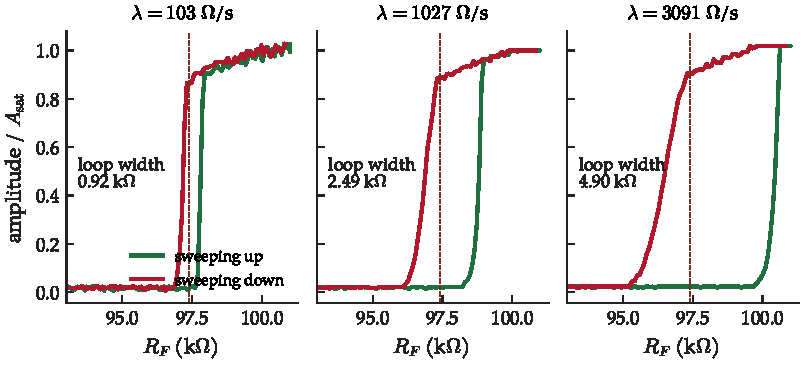
\includegraphics[width=\linewidth]{fig_s2_loops}
  \caption[Stage 2: hysteresis loops at three rates]{Stage 2: cycle-averaged amplitude against $\RF$,
  up (green) and down (red). Dashed: measured threshold.}
  \label{fig:s2-loops}
\end{figure}

\begin{figure}[!htb]
  \centering
  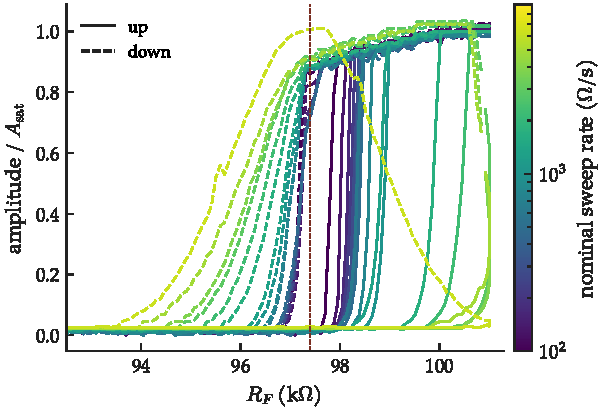
\includegraphics[width=0.52\linewidth]{fig_s2_allloops}
  \caption[Stage 2: loops for all 17 rates]{Stage 2: all 17 loops, coloured by rate (solid up, dashed
  down).}
  \label{fig:s2-allloops}
\end{figure}

\section{What this stage taught us}\label{sec:s2-learned}

\begin{learned}
\begin{itemize}[leftmargin=1.2em]
  \item \textbf{Criteria 1 and 2 hold on hardware}: a $\sqrt{\lambda}$ lag in both directions, with
        $k_{\mathrm{off}}$ within one standard error of the prediction.
  \item \textbf{Repeatable}: successive cycles agree to tens of ohms.
  \item \textbf{Real threshold $\Gc\approx3.07$}, measured by the slow-rate limit.
  \item \textbf{A first critical rate} near \SI{4}{\kilo\ohm\per\second}, set by the $\sqrt{\lambda}$ law
        and the sweep range.
\end{itemize}
\end{learned}

A lag, however, is not tipping: every cycle returned to the same quiet state. Criterion~3 needs a change
of the \emph{long-time state}, which required rates beyond the bench in this configuration, so we turned
to simulation.
